\documentclass{standalone}
\usepackage[ngerman]{babel}
% https://tex.stackexchange.com/questions/570303/use-blacktriangleright-as-itemize-label
\usepackage{amssymb} % for black triangleright

\renewcommand{\labelitemi}{$\textcolor{SwitchColor}{\bullet}$}
\renewcommand{\labelitemii}{$\textcolor{SwitchColor}{\blacktriangleright}$}
\renewcommand{\labelitemiii}{$\textcolor{SwitchColor}{\blacksquare}$}
\renewcommand{\labelitemiv}{$\textcolor{SwitchColor}{\blacksquare}$}

% https://tex.stackexchange.com/questions/525959/prevent-latex-from-stretching-math
\setlength{\thinmuskip}{1\thinmuskip}
\setlength{\medmuskip}{1\medmuskip}
\setlength{\thickmuskip}{1\thickmuskip}

\usepackage{tikzit}
\input{graph_theory.tikzstyles}
% \newenvironment{resettikz}{\pgfsetlayers{nodelayer,edgelayer}\tikzset{every node/.style={fill opacity=1.0, draw opacity=1.0}}}{}
\newenvironment{resettikz}{\tikzset{every node/.style={fill opacity=1.0, draw opacity=1.0}}}{}

\usepackage{array}
\usepackage{booktabs}
\usepackage{boldline}

\usepackage{tabularray}

\usepackage{subcaption}

\usepackage{csquotes}
\usepackage{xcolor}
% \usepackage{anyfontsize}
\usepackage[export]{adjustbox}
% \usepackage[]{enumitem}
\usepackage{nicematrix}
\usepackage{tikz}
\usetikzlibrary{arrows.meta,positioning}
\usetikzlibrary{graphs}
\usetikzlibrary{patterns}
\usetikzlibrary{shadings}
\usetikzlibrary{mindmap, shadows, backgrounds} % , calc

\definecolor{PrimaryColor}{HTML}{0B64A0}
\definecolor{PrimaryColorDimmed}{HTML}{A2D7F3}
\definecolor{SecondaryColor}{HTML}{6FC1EC}
\definecolor{SecondaryColorDimmed}{HTML}{CEEAF9}
\colorlet{BoxColor}{gray!10!white}

\usepackage[style=numeric]{biblatex}
\addbibresource{./My Library.bib}

\usepackage[allbordercolors=PrimaryColor, pdfborder={0 0 .2}]{hyperref}

% colored bold
% \newcommand\alert[1]{\textcolor{SwitchColor}{\textbf{#1}}}
\newcommand\alert[1]{\textcolor{SwitchColor}{#1}}

\newlength{\leveldistance}
\setlength{\leveldistance}{20cm}

\begin{document}
  \begin{tikzpicture}[
      auto,
      huge mindmap,
      fill opacity=0.6,
      draw opacity=0.8,
      concept color = PrimaryColorDimmed,
      every annotation/.style={fill=BoxColor, draw=none, align=center, fill = BoxColor, text width = 2cm},
      grow cyclic,
      level 1/.append style = {
        concept color=SecondaryColorDimmed,
        level distance=\leveldistance,
        sibling angle=360/\the\tikznumberofchildren,
        % https://tex.stackexchange.com/questions/501240/trying-to-use-the-array-environment-inside-a-tikz-node-with-execute-at-begin-no
        execute at begin node=\definecolor{SwitchColor}{named}{SecondaryColor},
      },
      level 2/.append style = {
        concept color=PrimaryColorDimmed,
        level distance=\leveldistance / 2,
        sibling angle=30,
        execute at begin node=\definecolor{SwitchColor}{named}{PrimaryColor},
      },
      level 3/.append style = {
        concept color=SecondaryColorDimmed,
        level distance=\leveldistance / 3,
        execute at begin node=\definecolor{SwitchColor}{named}{SecondaryColor},
      },
      level 4/.append style = {
        concept color=PrimaryColorDimmed,
        level distance=\leveldistance / 4,
        execute at begin node=\definecolor{SwitchColor}{named}{PrimaryColor},
      },
      level 5/.append style = {
        concept color=SecondaryColorDimmed,
        level distance=\leveldistance / 5,
        execute at begin node=\definecolor{SwitchColor}{named}{SecondaryColor},
      },
      level 6/.append style = {
        concept color=PrimaryColorDimmed,
        level distance=\leveldistance / 6,
        execute at begin node=\definecolor{SwitchColor}{named}{PrimaryColor},
      },
      level 7/.append style = {
        concept color=SecondaryColorDimmed,
        level distance=\leveldistance / 7,
        execute at begin node=\definecolor{SwitchColor}{named}{SecondaryColor},
      },
      level 8/.append style = {
        concept color=PrimaryColorDimmed,
        level distance=\leveldistance / 8,
        execute at begin node=\definecolor{SwitchColor}{named}{PrimaryColor},
      },
      concept connection/.append style = {
        color = BoxColor,
      },
  ]
  % damit Annotationen nicht auch eine Drop Shadow erhalten
  \begin{scope}[
      every node/.style = {concept, circular drop shadow}, % draw=none
      every child/.style={concept},
    ]
  \node (ti) at (current page.center) {Technische Informatik}
    child {
      node {Kodierung von Zeichen}
      child {
        node {Code, Codewörter
          \resizebox{\textwidth}{!}{
            \begin{minipage}[t]{10cm}
              \begin{itemize}
                \item Menge der \alert{Codewörter}: $c(A):=\left\{w\in\{0,1\}^{*}\;\right|\exists a\in A:c(a)=w\}$
                \item Eine Abbildung $c:{A}\rightarrow\{0,1\}^{*}$ oder $c:A\to\{0,1\}^{n}$ heißt \alert{Code}, falls $c$ injektiv ist 
              \end{itemize}
            \end{minipage}
          }
        }
        child {
          node {Alphabete, Wörter, Zeichen
            \resizebox{\textwidth}{!}{
              \begin{minipage}[t]{10cm}
                \begin{itemize}
                  \item nichtleeres Menge $A=\left\{a_{1},\dots,a_{m}\right\}$ heißt (endliches) \alert{Alphabet} der Größe $m$
                  \begin{itemize}
                    \item $a_1,\ldots, a_m$ heißen \alert{Zeichen} des Alphabets
                    \item $A^{*}=\{w\mid w=b_{1}\dots b_{n}\;m i t\;n\in\mathbb{N},\forall i\;m i t\;1\leq i\leq n:b_{i}\in A\}$ ist die \alert{Menge aller endlichen Wörter} über dem Alphabet $A$
                    \item $|b_1\ldots b_n| := n$ heißt Länge des Wortes $b_1\ldots b_n$
                    \item das Wort der Länge $0$ wird mit $\epsilon$
                  \end{itemize}
                \end{itemize}
              \end{minipage}
            }
          }
        }
        child {
          node {Codes fester Länge
            \resizebox{\textwidth}{!}{
              \begin{minipage}[t]{10cm}
                \begin{itemize}
                  \item $c:A\to\{0,1\}^{n}$ heißt \alert{Code fester Länge}
                  \begin{itemize}
                    \item für einen Code $c:A\to\{0,1\}^{n}$ fester Länge gilt: $n \ge \lceil log_2(m)\rceil$
                    \item ist $n=\lceil log_{2}m\rceil+r$ mit $r > 0$, so können die $r$ zusätzlichen Bits zum Test auf \alert{Übertragungsfehler} verwendet werden
                    \item Die Kodierung eines jeden Zeichens besteht aus $n$ Bits
                    \item einfach zu behandeln, unter Umständen wird faber mehr Speicherplatz gebraucht als nötig
                  \end{itemize}
                \end{itemize}
              \end{minipage}
            }
          }
          child {
            node {ASCII
              \resizebox{\textwidth}{!}{
                \begin{minipage}[t]{8cm}
                  \begin{itemize}
                    \item American Standard Code for Information Interchange
                    \item 7 Bits (es gibt Erweiterungen mit 8 Bits)
                  \end{itemize}
                  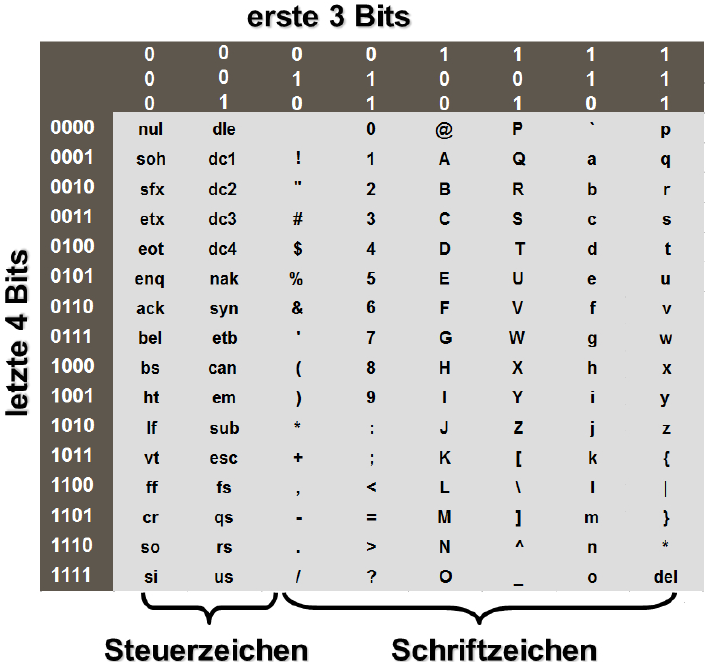
\includegraphics[width=0.5\textwidth, center]{./figures/ascii.png}
                \end{minipage}
              }
            }
          }
          child {
            node {EBCDIC
              \resizebox{\textwidth}{!}{
                \begin{minipage}[t]{8cm}
                  \begin{itemize}
                    \item Extended Binary Coded Decimal Interchange Code
                    \item 8 Bits
                  \end{itemize}
                \end{minipage}
              }
            }
          }
          child {
            node {Unicode
              \resizebox{\textwidth}{!}{
                \begin{minipage}[t]{8cm}
                  \begin{itemize}
                    \item 16 Bits
                  \end{itemize}
                \end{minipage}
              }
            }
          }
        }
        child {
          node {Häufigkeits-abhängige Codes
            \resizebox{\textwidth}{!}{
              \begin{minipage}[t]{8cm}
                \begin{itemize}
                  \item \alert{Ziel} ist die Reduktion der Länge einer Nachricht durch Wahl \alert{verschieden lange Codewörter} für die verschiedenen Zeichen eines Alphabets
                  \item häufiges Zeichen $\rightarrow$ kurzer Code
                  \item seltenes Zeichen $\rightarrow$ langer Code
                  % \item Häufigkeitsverteilung ist bekannt $\rightarrow$ \alert{statische Kompression}
                  % \item Häufigkeitsverteilung ist nicht bekannt $\rightarrow$ \alert{dynamische Kompression}
                \end{itemize}
              \end{minipage}
            }
          }
          child {
            node {Präfixcodes
              \resizebox{\textwidth}{!}{
                \begin{minipage}[t]{8cm}
                  \begin{itemize}
                    \item $a_{1}\ldots a_{p}\in A^{*}$ über einem Alphabet $A$ der Größe $m$ heißt \alert{Präfix} von $b_{1}\ldots b_{l}\in A^{*}$, falls $p\le l$ und $\forall i: a_i=b_i$, $1\le i\le p$
                    \item Ein Code $c:A\rightarrow\{0,1\}^{*}$ heißt \alert{Präfixcode}, falls es kein Paar $i,j\in\{\,1,\ldots,m\}$ gibt, so dass $c(a_i)$ Präfix von $c(a_j)$
                    \item Bei Präfixcodes können Wörter über $\{0, 1\}$ eindeutig dekodiert werden. (Sie entsprechen Binärbäumen mit codierten Zeichen an den Blättern.)
                  \end{itemize}
                \end{minipage}
              }
            }
            child {
              node {Huffman
                \resizebox{\textwidth}{!}{
                  \begin{minipage}[t]{10cm}
                    \begin{itemize}
                      \item \alert{Vorgehen:}
                      \begin{enumerate}
                        \item Baue binären Baum, indem die beiden kleinsten Häufigkeiten jeweils zu einem neuen Knoten addiert werden
                        \item Markiere die linken Kanten mit $0$ und die rechten Kanten mit $1$
                      \end{enumerate}
                      \item Huffman-Code ist ein bzgl. mittlerer Codelänge optimaler \alert{Präfixcode} (unter Voraussetzung einer bekannten Häufigkeitsverteilung)
                      \item Kommt als Teilschritt z.B. in MP3 oder JPEG vor.
                    \end{itemize}
                    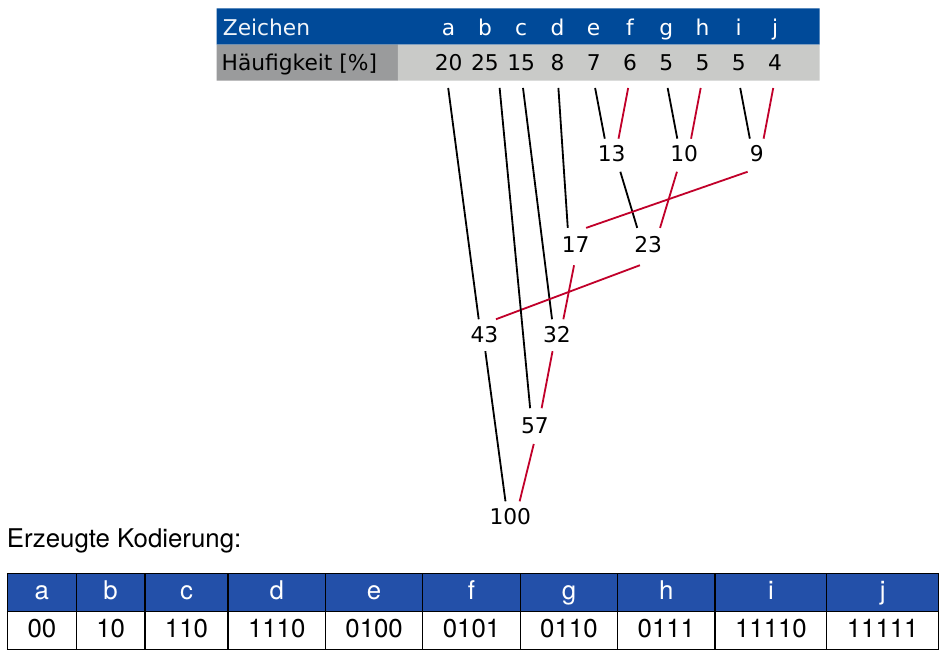
\includegraphics[width=0.8\textwidth, center]{./figures/huffman_codierung.png}
                  \end{minipage}
                }
              }
            }
          }
        }
      }
    }
    child {
      node {Kodierung von Zahlen}
      child {
        node {Zahlensystem
          \resizebox{\textwidth}{!}{
            \begin{minipage}[t]{12cm}
              \begin{itemize}
                \item $S = (b, Z, \delta)$, 
                \begin{itemize}
                  \item \alert{Basis} $b\in\mathbb{N}: b\ge 1$ des Stellenwertsystems mit welcher für jede \alert{Stelle} $i$ der \alert{Stellenwert} $b^i$ berechnet wird
                  \begin{itemize}
                    \item bei der $n$-stelligen Binärdarstellung einer Zahl werden dem \alert{LSB} und \alert{MSB} jeweils die Stellenwerte $b^0$ und $b^{n-1}$ zugeordnet
                  \end{itemize}
                  \item $b$-elementige \alert{Ziffernmenge} von Symbolen $Z$, die \alert{Ziffern}
                  \item \alert{Ziffernwertigkeit} $\delta: Z\rightarrow \{0, 1, \ldots, b-1\}$ ordnet jeder \alert{Ziffer} bzw. Symbol ihre \alert{Wertigkeit} zu
                  \begin{itemize}
                    \item im z.B. \alert{Hexadezimalsystem} werden den sechzehn Ziffern $0, 1, 2, 3, 4, 5, 6, 7, 8, 9, A, B, C, D, E$ und $F$ jeweils die Werte der Dezimalzahlen von $0$ bis $15$ zugeordnet.
                  \end{itemize}
                \end{itemize}
                \item verwendetes Zahlensystem wird durch Anhängen der \alert{Basis als Index} an die Ziffernfolge ${d_{n-1}\ldots d_{0}}_b$ vermittelt
                \item \alert{Eselsbrücken fürs Hexadezimalsystem:} \alert{C}wölf, \alert{D}reizehn, \alert{F}ünfzehn
                  % \begin{itemize}
                  %   \begin{itemize}
                  %   \end{itemize}
                  %     % $(z_i)_{i=0,\ldots,n}$
                  %     % $z\ =\ z_{n-1}\ldots z_{0}$
                  % \end{itemize}
                  % \begin{itemize}
                  %     \begin{itemize}
                  %     \end{itemize}
                  % \end{itemize}
              \end{itemize}
            \end{minipage}
          }
        }
        child {
          node {Warum sich manche Zahlensystem einfacher ineinander unformen lassen
            \resizebox{\textwidth}{!}{
              \begin{minipage}[t]{8cm}
                \begin{align*}
                  ba_{16} &= b_{16} \cdot 16^1 + a_{16} \cdot 16^0\\
                          &= 13_{8} \cdot 16^1 + 12_{8} \cdot 16^0\\
                          &= (1_{8} \cdot 8^1 + 3_{8}) \cdot 16^1 + (1_{8} \cdot 8^1+  2_{8}) \cdot 16^0\\
                          &= (1_{8} \cdot 8^1 + 3_{8}) \cdot (8 \cdot 2)^1 + (1_{8} \cdot 8^1+  2_{8}) \cdot (8 \cdot 2)^0\\
                          &= 2_{8} \cdot 8^2 + 6_{8} \cdot 8^1 + 1_{8} \cdot 8^1 \cdot (8 \cdot 2)^0 + 2_{8} \cdot (8 \cdot 2)^0\\
                          &= 2_{8} \cdot 8^2 + 7_{8} \cdot 8^1 + 2_{8} \cdot 1 = 272_{8} \\
                  ba_{16} &= b_{16} \cdot 16^1 + a_{16} \cdot 16^0\\
                          &= 1011_{2} \cdot (2^4)^1 + 1010_{2} \cdot (2^4)^0 = 10111010_{2}
                \end{align*}
              \end{minipage}
            }
          }
        }
        child {
          node {Natürliche Zahl
            \resizebox{\textwidth}{!}{
              \begin{minipage}[t]{10cm}
                \begin{itemize}
                  \item \alert{positiver Wert} $\displaystyle \langle d\rangle\ =\ \sum_{i=0}^{n-1} \delta(d_{i})\cdot b^{i}$ einer \alert{nicht-negativen Natürlichen Zahl}, wobei $d=d_{n-1}\ldots d_0$ mit $d_i\in Z$ eine \alert{Folge} von $n$ \alert{Ziffern} bzw. Symbolen ist
                \end{itemize}
              \end{minipage}
            }
          }
        }
        child {
          node {Festkommazahl
            \resizebox{\textwidth}{!}{
              \begin{minipage}[t]{12cm}
                \begin{itemize}
                  \item eine endliche Folge von Ziffern aus einem Zahlensystem zur Basis $b$ mit Ziffernmenge $Z$
                  \item \alert{positiver Wert} $\displaystyle \langle d\rangle=\sum_{i=-k}^{n-1}\delta(d_{i})\cdot b^{i}$ einer \alert{nicht-negativen Festkommazahl}, wobei $d=d_{n-1}\ldots d_0\ldots d_{-k}$ mit $d_i\in Z$
                    \begin{itemize}
                      \item \alert{die Anzahl der Nachkommastellen ist fest:} $\langle d_{n-1}\ldots d_0 d_{-1}\ldots d_{-k}\rangle \cdot 2^{-k} = \langle d_{n-1}\ldots d_0\textcolor{PrimaryColor}{.}d_{-1}\ldots d_{-k}\rangle$
                      \item Beispiel 3-Bit Festkommazahlen mit $n=1$ und $k=2$:
                        \begin{table}
                          \raggedright
                          \begin{tblr}{
                              cells = {c, BoxColor},
                              column{1} = {PrimaryColor,fg=white},
                            }
                            $d$                & 0.00 & 0.01 & 0.10 & 0.11 & 1.00 & 1.01 & 1.10 & 1.11 \\
                            $\langle d\rangle$ & 0.0  & 0.25 & 0.5  & 0.75 & 1.0  & 1.25 & 1.5  & 1.75 \\
                          \end{tblr}
                        \end{table}
                    \end{itemize}
                    \item Probleme:
                    \begin{itemize}
                      \item keine ganz großen bzw. kleinen Zahlen darstellbar
                      \item weitere Probleme \href[page=152]{./Technische_Informatik_all_in_one_with_go_back.pdf}{hier} erklärt
                    \end{itemize}
                \end{itemize}
                \begin{figure}
                  \begin{subfigure}{0.4\textwidth}
                    \centering
                    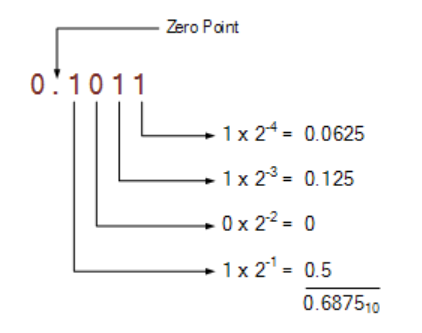
\includegraphics[width=0.8\linewidth]{figures/binary_fraction.png}
                    \caption{Binärbrüche}
                    \label{fig:binaryfraction}
                  \end{subfigure}
                  \begin{subfigure}{0.4\textwidth}
                    \centering
                    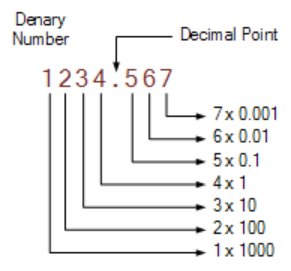
\includegraphics[width=0.6\linewidth]{figures/decimal_fraction.png}
                    \caption{Dezimalbrüche}
                    \label{fig:decimalfraction}
                  \end{subfigure}
                \end{figure}
              \end{minipage}
            }
          }
          child {
            node {Negative Festkommazahl
              \resizebox{\textwidth}{!}{
                \begin{minipage}[t]{8cm}
                  \begin{itemize}
                    \item mehrere mögliche Darstellungen für \alert{negative Festkommazahlen}, wobei $d=d_{n}d_{n-1}\ldots d_0\ldots d_{-k}$ mit $\forall i\langle n:d_i\in Z$ und $d_n\in\{0, 1\}$:
                    \begin{itemize}
                      \item $n+1$ \alert{Vorkommastellen}, wovon allderings ein Bit ein \alert{Vorzeichenbit} ist und $n$ Bits \alert{Nicht-Vorzichenbits} sind
                      \item $k$ \alert{Nachkommastellen}
                    \end{itemize}
                    \item ein Vorteil von Einerkomplement- und Zweierkomplement-Darstellung ist, dass sie \alert{zyklisch} sind:
                      \begin{align*}
                        [01.1]_2 + 0.5 &= [10.0]_2 &\text{(nach } 1.5 \text{ geht es mit } {-}2 \text{ weiter)}\\
                        [01.1]_1 + 0.5 &= [10.0]_1 &\text{(nach } 1.5 \text{ geht es mit } {-}1.5 \text{ weiter)}\\
                      \end{align*}
                  \end{itemize}
                \end{minipage}
              }
            }
            child {
              node {Betrag und Vorzeichen Darstellung
                \resizebox{\textwidth}{!}{
                  \begin{minipage}[t]{12cm}
                    \begin{itemize}
                      \item \alert{potentiell negativer Wert} $\displaystyle[d]_{BV} = (-1)^{d_n}\sum_{i=0}^{n-1}\delta(d_i)2^i$ in \alert{Darstellung durch Betrag und Vorzeichen}
                        \begin{itemize}
                          \item Beispiel 3-Bit Festkommazahlen mit Vorzeichenbit, $n=1$ und $k=1$:
                            \begin{table}
                              \raggedright
                              \begin{tblr}{
                                  cells = {c, BoxColor},
                                  column{1} = {PrimaryColor,fg=white},
                                }
                                $d$        &  11.1  & 11.0 & 10.1 & 10.0 / 00.0 & 00.1 & 01.0 & 01.1 \\
                                $[d]_{BV}$ & -1.5 & -1.0 & -0.5 & 0.0 & 0.5 & 1.0  & 1.5 \\
                              \end{tblr}
                            \end{table}
                        \end{itemize}
                    \end{itemize}
                  \end{minipage}
                }
              }
            }
            child {
              node {Radixkomplement
                \resizebox{\textwidth}{!}{
                  \begin{minipage}[t]{12cm}
                    \begin{itemize}
                      \item Das \alert{Radix-Komplement} (r's Komplement) von einer Zahl y mit $n-$Ziffern mit Radix $b$:
                        \begin{equation*}
                          b^n-y
                        \end{equation*}
                      \item Es gibt auch ein \alert{verringertes Radix-Komplement} ((r-1)'s Komplement), und zwar:
                        \begin{equation*}
                          (b^n-1)-y
                        \end{equation*}
                        \cite{OnlineRechnerNumerischeKomplemente}
                      \item Das \alert{verringerte Radix-Komplement} kann man leicht erhalten, indem man einfach die Ziffern einer Zahl mit den Ziffern, die man benötigt um $Radix - 1$ zu erhalten, ersetzt. Zum Beispiel, dass verringerte Radix-Komplement für die 2-Ziffern Dezimalzahl $56$ ist $43$. Man kann das \alert{Radix-Komplement} einfach erhalten, indem man Eins zu dem verringerten Radix-Komplement addiert $43+1=44$
                      \item Im Dezimalzahlensystem ist das Radix-Komplement auch als \alert{Zehnerkomplement} (10'er Komplement) und das verringerte Radix-Komplement als \alert{Neunerkomplement} (9'er Komplement) bekannt
                      \item Im Binärsystem ist das Radix-Komplement als \alert{Zweierkomplement} (2'er Komplement) und das verringerte Radix-Komplement als \alert{Einerkomplement} (1'er Komplement) bekannt. Ein Einerkomplement kann man einfach durch das Umkehren von Bits einer Zahl erhalten. Zweierkomplemente werden in Computern für die Darstellung von negativen Ganzzahlen verwendet
                    \end{itemize}
                  \end{minipage}
                }
              }
              child {
                node {Komplementärverfahren (engl. Method of complements\cite{MethodComplements2023})
                  \resizebox{\textwidth}{!}{
                    \begin{minipage}[t]{12cm}
                      \begin{itemize}
                        \item Subtraktion als Addition berechnen. Beispiele:
                          \begin{align*}
                    &\begin{aligned}
                      622_{10} - 451_{10} \text{ ist } 622_{10} + (1000_{10} - 451_{10}) - 1000_{10} &= 622_{10} + (999_{10} - 451_{10} + 1) - 1000_{10}\\
                                                                                                     &= 622_{10} + 549_{10} - 1000_{10}\\
                                                                                                     &= 1171_{10} - 1000_{10} = 171_{10}
                    \end{aligned}\\[0.25cm]
                    &\begin{aligned}
                      110_{2} - 011_{2} \text{ ist } 110_{2} + (1000_{2} - 011_{2}) - 1000_{2} &= 110_{2} + (999_{2} - 011_{2} + 1) - 1000_{2}\\
                                                                                               &= 110_{2} + 101_{2} - 1000_{2}\\ 
                                                                                               &= 1011_{2} - 1000_{2} = 11_{2}
                    \end{aligned}
                          \end{align*}
                      \end{itemize}
                    \end{minipage}
                  }
                }
              }
              child {
                node {Einer-Komplement Darstellung
                  \resizebox{\textwidth}{!}{
                    \begin{minipage}[t]{14cm}
                      \begin{itemize}
                        \item \alert{potentiell negativer Wert} $\displaystyle[d]_{1} = \sum_{i=0}^{n-1}\delta(d_i) 2^i - \delta(d_n)(2^n-2^{-k})$ in \alert{Einerkomplement-Darstellung}
                          \begin{itemize}
                            \item Beispiel 3-Bit Festkommazahlen mit Vorzeichenbit, $n=1$ und $k=1$:
                              \begin{table}
                                \raggedright
                                \begin{tblr}{
                                    cells = {c, BoxColor},
                                    column{1} = {PrimaryColor,fg=white},
                                  }
                                  $d$     & 10.0 & 10.1 & 11.0 & 11.1 / 00.0 & 00.1 & 01.0 & 01.1 \\
                                  $[d]_1$ & -1.5  & -1.0 & -0.5  & 0.0 & 0.5 & 1.0  & 1.5 \\
                                \end{tblr}
                              \end{table}
                          \end{itemize}
                      \end{itemize}
                      \begin{itemize}
                        \item im Negativen hat eine Folge mit mehr $1$en anders als im Positiven betragsmäßig eine kleineren Wert, denn umso mehr $1$en da sind, umso größer wird die Summe $\sum_{i=0}^{n-1}\delta(d_i)2^i$ und umso mehr kann von der subtrahierten größten positiven Zahl $2^n-1$ ausgeglichen werden
                        \item um den Wert einer negativen Dezimalzahl binär darzustellen gibt es 2 Methoden:
                          \begin{itemize}
                            \item mit größtmöglichen positven Zahl anfangen $-(2^n-1)$ und überlegen, welche $2$er Potenzen (Stellenwerte) man draufaddieren muss, um die gewünschte Zahl zu erhalten und an den entsprechenden Bits, die diesen $2$er Potenzen entsprechen $1$en setzen
                            \item die passende Ziffernfolge wie gewohnt erstellen, aber mit vertauschten $1$en und $0$en und das Vorzeichenbit ist eine $1$
                          \end{itemize}
                      \end{itemize}
                    \end{minipage}
                  }
                }
                child {
                  node {Inversion
                    \resizebox{\textwidth}{!}{
                      \begin{minipage}[t]{8cm}
                        \begin{itemize}
                          \item $[a']_1 = -[a]_1$
                        \end{itemize}
                      \end{minipage}
                    }
                  }
                }
              }
              child {
                node {Zweier-Komplement Darstellung
                  \resizebox{\textwidth}{!}{
                    \begin{minipage}[t]{14cm}
                      \begin{itemize}
                        \item man springt einen kleisten Zahlenabstand weiter wenn das Vorzeichenbit $1$ ist als beim Einerkomplement
                        \item \alert{potentiell negativer Wert} $\displaystyle[d]_{2} = \sum_{i=0}^{n-1}\delta(d_i)2^i - \delta(d_n)2^n$ in \alert{Zweierkomplement-Darstellung}
                          \begin{itemize}
                            \item Beispiel 3-Bit Festkommazahlen mit Vorzeichenbit, $n=1$ und $k=1$:
                              \begin{table}
                                \raggedright
                                \begin{tblr}{
                                    cells = {c, BoxColor},
                                    column{1} = {PrimaryColor,fg=white},
                                  }
                                  $d$                & 10.0 & 10.1 & 11.0 & 11.1 & 00.0 & 00.1 & 01.0 & 01.1 \\
                                  $[d]_2$ & -2  & -1.5 & -1.0  & -0.5 & 0.0  & 0.5 & 1.0  & 1.5 \\
                                \end{tblr}
                              \end{table}
                          \end{itemize}
                      \end{itemize}
                      \begin{itemize}
                        \item genauso wie beim Einerkomplment bedeuten mehr $1$en im Negativen einen betragsmäßig kleineren Wert
                        \item um den Wert einer negativen Dezimalzahl binär darzustellen gibt es 2 Methoden
                          \begin{itemize}
                            \item mit der größtmöglichen positven Zahl + kleinmöglichen positven Zahl ungleich $0$ anfangen $-(2^n)$ und überlegen, welche $2$er Potenzen (Stellenwerte) man draufaddieren muss, um die gewünschte Zahl zu erhalten und an den entsprechenden Bits, die diesen $2$er Potenzen entsprechen $1$en setzen
                            \item die passende Ziffernfolge wie gewohnt erstellen, aber die kleinstmögliche positve Zahl ungleich $0$ wird als Startwert genommen und die $1$en und $0$en sind vertauscht, sowie das Vorzeichenbit ist eine $1$
                          \end{itemize}
                        \item wenn man die kleinste negative Zahl komplementiert: $[10.0]_2' = [01.1]_1 + 0.5 = [10.0]_2$, dann erhält man erneut die kleinste negative Zahl. Das passt auch ganz gut, da die kleinste negative Zahl im Zweierkomplement keine komplementäre positive Zahl hat. Folglich auch hier: $[a]_2 + [a']_2 + 2^{-k} = [1.00]_2 + [0.11]_2 + 0.5 = -2 + 1.5 + 0.5 = 0$ für $a$ kleinste Zweierkomplement-Zahl
                      \end{itemize}
                    \end{minipage}
                  }
                }
                child {
                  node {Addition von Zweierkomplementzahlen
                    \resizebox{\textwidth}{!}{
                      \begin{minipage}[t]{12cm}
                        \begin{itemize}
                          \item \href[page=359]{/home/areo/Documents/Studium/Summaries/Technische_Informatik/Technische_Informatik_all_in_one_with_go_back.pdf}{reference}
                          \item \href[page=360]{/home/areo/Documents/Studium/Summaries/Technische_Informatik/Technische_Informatik_all_in_one_with_go_back.pdf}{Überlauftest}
                        \end{itemize}
                      \end{minipage}
                    }
                  }
                }
                child {
                  node {Subtraktion von Zweierkomplementzahlen
                    \resizebox{\textwidth}{!}{
                      \begin{minipage}[t]{12cm}
                        \begin{itemize}
                          \item \href[page=363]{/home/areo/Documents/Studium/Summaries/Technische_Informatik/Technische_Informatik_all_in_one_with_go_back.pdf}{reference}
                        \end{itemize}
                      \end{minipage}
                    }
                  }
                }
                child {
                  node {Inversion
                    \resizebox{\textwidth}{!}{
                      \begin{minipage}[t]{8cm}
                        \begin{itemize}
                          \item $[a']_2 + 1 = -[a]_2$
                        \end{itemize}
                      \end{minipage}
                    }
                  }
                }
              }
            }
          }
        }
        child {
          node {Gleitkommazahl
            \resizebox{\textwidth}{!}{
              \begin{minipage}[t]{16cm}
                \begin{itemize}
                  \item Darstellung \alert{negativer Gleitkommazahlen}, wobei $\underbrace{d_n}_{sign} \underbrace{d_{n-1} \ldots d_0}_{exponent} \underbrace{d_{-1}\ldots d_{-k}}_{fraction / mantissa}$ mit exponent, fraction bits und sign bit aus $\{0, 1\}$:
                    \begin{itemize}
                      \item \alert{varierende Anzahl von Nachkommastellen} im Gegensatz zu Festkommazahlen
                      \item \alert{Normalisierte Zahlen:} $(-1)^{d_n} \cdot \langle 1 d_{-1}\ldots d_{-k}\rangle \cdot 2^{-k+\langle d_{n-1}\ldots d_{0}\rangle-(2^{n-1}-1)} = (-1)^{sign} \times (1 + fraction) \times 2^{exponent - bias}$
                        \begin{itemize}
                          \item \alert{Bias:} $2^{n-1} - 1 = \dfrac{2^2}{2} - 1 = 2 - 1 = \boxed{01_{2}}$, \alert{größter, kleinster Exponent:} $11_2 - 01_2 = \boxed{10_2}$, $01_2 - 01_2 = \boxed{00_2}$
                          \item \alert{Betragsmäßig kleinste, größte Zahl:} $\pm 1.0\times 2^{1-1} =\pm 1.0$ ($\boxed{\frac{0}{1}\mid 01\mid 0}$), $\pm 1.5 \times 2^{2-1} =\pm 3$ ($\boxed{\frac{0}{1}\mid 10\mid 1}$)
                        \end{itemize}
                      \item \alert{Denormalisierte Zahlen:} $(-1)^{d_n} \cdot \langle 0 d_{-1}\ldots d_{-k}\rangle \cdot 2^{-k+\langle d_{n-1}\ldots d_{0}\rangle-(2^{n-1}-2)} = (-1)^{sign} \times (0 + fraction) \times 2^{-bias}$
                        \begin{itemize}
                          \item \alert{Bias:} $2^{n-1} - 2 = \dfrac{2^2}{2} - 2 = 2 - 2 = \boxed{00_{2}}$, \alert{einziger Exponent:} $00_2 - 00_2 = \boxed{00_2}$
                          \item \alert{Betragsmäßig kleinste, größte Zahl:} $0.0 \times 2^{0-0} = 0$ ($\boxed{\frac{0}{1}\mid 00\mid 0}$), $\pm 0.5 \times 2^{0-0} =\pm 0.5$ ($\boxed{\frac{0}{1}\mid 00\mid 1}$)
                        \end{itemize}
                        \begin{itemize}
                          \item $1 \textcolor{PrimaryColor}{.}d_{-1}\ldots d_{-k}$ wird als \alert{normalized significand} bezeichnet
                          \item $0 \textcolor{PrimaryColor}{.}d_{-1}\ldots d_{-k}$ wird als \alert{normed significand} bezeichnet
                        \end{itemize}
                      \item der \alert{Exponent} ist immer als \alert{nicht-negative} Natürliche Zahl zu interpretieren, die \alert{Mantissa} ist immer als \alert{nicht-negativer Bruch} zu interpretieren, also mit $2^{-k}$ zu multiplizieren
                      \item der \alert{Bias} macht den $encoded\_exponent$ immer \alert{positiv}
                        \begin{itemize}
                          \item $encoded\_exponent = real\_exponent + bias$
                          \item $real\_exponent = encoded\_exponent - bias$
                        \end{itemize}
                      \item \alert{Zero:} $\boxed{\frac{0}{1}\mid 00\mid 0}$, \alert{Infinity:} $\boxed{\frac{0}{1}\mid 11\mid 0}$, \alert{NaN:} $\boxed{\frac{0}{1}\mid 11\mid 1}$
                      \item Beispiel 4-Bit Gleitkommazahl mit Vorzeichenbit, $2$ Exponentbits und Mantissabit:
                        {\tiny
                          \begin{table}
                            \raggedright
                            \begin{tblr}{
                                cells = {c, BoxColor},
                                column{1} = {PrimaryColor,fg=white},
                              }
                              $d$      & $1\mid00\mid0$ & $1\mid00\mid1$ & $1\mid01\mid0$  & $1\mid01\mid1$ & $1\mid10\mid0$ & $1\mid10\mid1$ & $1\mid11\mid0$ & $1\mid11\mid1$ \\
                              $[d]_{GK}$  & 0.0  & -0.5 & -1.0 & -1.5 & -2.0  & -3.0 & $-\infty$  & NaN \\
                              $d$ als BV  & 0.0            & -0.1           & -1.0           & -1.1           & -10.0          & -11.0          & -              & -              \\
                            \end{tblr}
                          \end{table}
                          \begin{table}
                            \raggedright
                            \begin{tblr}{
                                cells = {c, BoxColor},
                                column{1} = {PrimaryColor,fg=white},
                              }
                              $d$      & $0\mid00\mid0$ & $0\mid00\mid1$ & $0\mid01\mid0$ & $0\mid01\mid1$ & $0\mid10\mid0$ & $0\mid10\mid1$ & $0\mid11\mid0$ & $0\mid11\mid1$ \\
                              $[d]_{GK}$  & 0.0  & 0.5 & 1.0 & 1.5 & 2.0  & 3.0 & $\infty$  & NaN \\
                              $d$ als BV  & 0.0            &  0.1           &  1.0           & 1.1            & 10.0           & 11.0           & -              & -              \\
                              % 0.0, 0.5, 1.0, 1.5, 2.0, 3.0, 4.0, 6.0
                            \end{tblr}
                          \end{table}
                        }
                      \item Beispiel \alert{ohne angepassten Bias} ($-2$) für \alert{Denormalisierte Zahlen} mit 4-Bit Gleitkommazahl mit Vorzeichenbit, $2$ Exponentbits und Mantissabit:
                        {
                          \tiny
                          % \begin{table}
                          %   \raggedright
                          %   \begin{tblr}{
                          %       cells = {c, BoxColor},
                          %       column{1} = {PrimaryColor,fg=white},
                          %     }
                          %     $d$      & $1\mid00\mid0$ & $1\mid00\mid1$ & $1\mid01\mid0$  & $1\mid01\mid1$ & $1\mid10\mid0$ & $1\mid10\mid1$ & $1\mid11\mid0$ & $1\mid11\mid1$ \\
                          %     $[d]_{GK}$  & 0.0  & -0.25& -1.0 & -1.5 & -2.0  & -3.0 & $\infty$  & NaN \\
                          %     $d$ als BV  & 0.0            & -0.01           & -1.0           & -1.1           & -10.0          & -11.0          & -              & -              \\
                          %   \end{tblr}
                          % \end{table}
                          \begin{table}
                            \raggedright
                            \begin{tblr}{
                                cells = {c, BoxColor},
                                column{1} = {PrimaryColor,fg=white},
                              }
                              $d$      & $0\mid00\mid0$ & $0\mid00\mid1$ & $0\mid01\mid0$ & $0\mid01\mid1$ & $0\mid10\mid0$ & $0\mid10\mid1$ & $0\mid11\mid0$ & $0\mid11\mid1$ \\
                              $[d]_{GK}$  & 0.0  & 0.25& 1.0 & 1.5 & 2.0  & 3.0 & $\infty$  & NaN \\
                              $d$ als BV  & 0.0            &  0.01           &  1.0           & 1.1            & 10.0           & 11.0           & -              & -              \\
                            \end{tblr}
                          \end{table}
                        }
                      \item Beispiel \alert{ohne um $-1$ geshifteten Bias} mit 4-Bit Gleitkommazahl mit Vorzeichenbit, $2$ Exponentbits und Mantissabit:
                        {
                          \tiny
                          %     \begin{table}
                          %       \raggedright
                          %       \begin{tblr}{
                          %           cells = {c, BoxColor},
                          %           column{1} = {PrimaryColor,fg=white},
                          %         }
                          %         $d$      & $1\mid00\mid0$ & $1\mid00\mid1$ & $1\mid01\mid0$  & $1\mid01\mid1$ & $1\mid10\mid0$ & $1\mid10\mid1$ & $1\mid11\mid0$ & $1\mid11\mid1$ \\
                          %           $[d]_{GK}$  & 0.0  & -0.25& -0.5 & -0.75 & -1.0  & -2.0 & $\infty$  & NaN \\
                          % % 0.0, 0.25, 0.5, 0.75, 1.0, 1.5, 2.0, 3.0
                          %           $d$ als BV  & 0.0            &  -0.01           &  -0.1           & -0.11            & -1.0           & -10.0           & -              & -              \\
                          %       \end{tblr}
                          %     \end{table}
                          \begin{table}
                            \raggedright
                            \begin{tblr}{
                                cells = {c, BoxColor},
                                column{1} = {PrimaryColor,fg=white},
                              }
                              $d$      & $0\mid00\mid0$ & $0\mid00\mid1$ & $0\mid01\mid0$ & $0\mid01\mid1$ & $0\mid10\mid0$ & $0\mid10\mid1$ & $0\mid11\mid0$ & $0\mid11\mid1$ \\
                              $[d]_{GK}$  & 0.0  & 0.25& 0.5 & 0.75 & 1.0  & 1.5 & $\infty$  & NaN \\
                              % 0.0, 0.25, 0.5, 0.75, 1.0, 1.5, 2.0, 3.0
                              $d$ als BV  & 0.0            &  0.01           &  0.1           & 0.11            & 1.0           & 1.1           & -              & -              \\
                            \end{tblr}
                          \end{table}
                        }
                        \begin{itemize}
                          \item es gibt mehr positive Exponenten als negative Exponenten 
                          \item die Zahl $1.0$ und damit viele Festkommazahlen mit so vielen Mantissa-Bits, wie für die Gleitkommazahl zu Verfügung stehen sind sehr einfach zu kodieren, da $(1+fraction) \cdot 2^{\sum_{i=0}^{n-2} 1 \cdot 2^i - (2^{n-1}-1)} = (1+fraction) \cdot 2^{2^{n-1}-1 - 2^{n-1}+1} = (1+fraction) \cdot 2^0 = (1+fraction)$
                        \end{itemize}
                      \item es gibt \alert{verschiedene Standards}, wie \alert{Bfloat16} ($1$ sign bit, $8$ exponent bits, $7$ fraction bits), \alert{Single-precision} ($1$ sign bit, $8$ exponent bits, $23$ fraction bits) und \alert{Double-precision} ($1$ sign bit, $11$ exponent bits, $52$ fraction bits), die sich in der \alert{Anzahl der Bits} für \alert{Exponent} und \alert{Mantissa} unterscheiden
                      \item \alert{Runden mit GRS-Bits:}
                        \begin{itemize}
                          \item mit GRS braucht man nur $3$ zusätzliche Bits und braucht so keinen großen und langsamen Addierer mit dem man die Berechnungen erstellt. Ohne GRS müsste man die Berechnungen mit allen Bits machen und am Ende runden
                          \item \alert{Guard und Round bit:} Zwei zusätzliche Bits die bei Berechnungen mit Gleitkommazahlen rechts angehängt werden, um die Rundungsgenauigkeit zu erhöhen
                          \item \alert{Sticky bit:} Zusätzliches Bits rechts der Bits Guard und Round, dass gesetzt wird, wann immer es Bits rechts davon gibt, die nicht $0$ sind
                          \item \alert{Ties to even:} Numbers exactly in the middle between two integer numbers (\enquote{ties}) are rounded towards the even number\\
                              \begin{minipage}{0.5\linewidth}
                                % \vspace{-0.25cm}
                                \begin{align*}
                                  0.5 \to 0,\\
                                  1.5 \to 2,\\
                                  2.5 \to 2
                                \end{align*}
                              \end{minipage}
                              \begin{minipage}{0.5\linewidth}
                                % \vspace{-0.75cm}
                                \begin{table}
                                  \centering
                                  \begin{tblr}{
                                      cells = {c, BoxColor},
                                      row{1} = {PrimaryColor,fg=white},
                                    }
                                    G & R & S & Ergebnis \\
                                      &     & 1/8 & 0.125 \\
                                      & 1/4 &     & 0.25  \\
                                      & 1/4 & 1/8 & 0.375 \\
                                    1/2 &     &     & 0.5   \\
                                    1/2 &     & 1/8 & 0.625 \\
                                    1/2 & 1/4 &     & 0.75  \\
                                    1/2 & 1/4 & 1/8 & 0.875
                                  \end{tblr}
                                \end{table}
                              \end{minipage}
                        \end{itemize}
  \end{itemize}
      \begin{itemize}
        \item the Anordnung, dass der \alert{Exponent} immer vor der \alert{Mantissa} steht und der Fakt, dass der kodierte Exponent positiv ist, ist so gewählt, damit man Gleitkommazahlen möglichst einfach vergleichen kann
        \item \alert{Festkommazahlen} haben eine \alert{kleinere Repräsentationsspanne}, da sie nur eine \alert{feste Anzahl an Nachkommastellen} haben. Gleitkommazahlen sind \alert{nicht gleichmäßig verteilt}, man hat eine sehr \alert{hohe Dichte kleiner Zahlen} nahe der $0$, neben einem schmallen Bereich nahe der $0$ mit gar keinen Zahlen.\\[0.25cm]
        \begin{figure}
          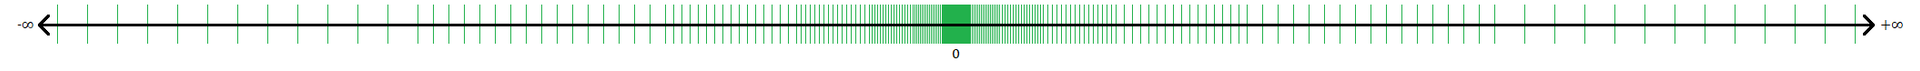
\includegraphics[width=\linewidth]{./figures/scaling.png}
          \caption{Verteilung von Gleitkommazahlen}
        \end{figure}
        \vspace{-0.5cm}
        \tiny
        \begin{table}
          \centering
          \begin{tblr}{
              cells = {c, white},
              column{1} = {PrimaryColor,fg=white},
            }
            $d[i]$      & 0.101 & 1.01 & 10.1 & 101 \\
            $\langle d[i]\rangle$  & 0.625  & 1.25 & 2.5 & 5 & \\
            $\langle d[i]\rangle - \langle d[i-1]\rangle$  & 0.3125 & 0.625 & 1.25 & 2.5 & \\
          \end{tblr}
          \caption{Abstände erhöhen sich exponentiel}
        \end{table}
      \end{itemize}
                \end{itemize}
              \end{minipage}
            }
          }
        }
      }
    }
    child {
      node {Mathematische Grundlagen
        \resizebox{\textwidth}{!}{
          \begin{minipage}[t]{12cm}
          \end{minipage}
        }
      }
      child {
        node {Groß-O-Notation
          \resizebox{\textwidth}{!}{
            \begin{minipage}[t]{12cm}
              \begin{itemize}
                \item Man will Funktionen irendwie vergleichen und das einzige sinnvolle was man vergleichen kann ist die \alert{Wachstumsrate}, denn für zwei Funktionen kann gleichzeitig gelten: $g = O(f)$, also $g$ wächst nicht stärker als $f$ und $g > f$, also $g$ ist überall echt größer als $f$
                \item Konstate Faktoren und Summanden $c \cdot x$ und $c + x$ sollen keine Rolle, aber es geht um \alert{Wachstumsrate}, Konstante Faktoren und Summanden spielen keine Rolle
                \item man interessiert sich meist nur für die kleinste/größtere untere/obere Grenze, z.B. wenn $f\in O(n)$ dann gilt automatisch auch $f\in O(n^2)$, aber man interessiert sich nur für die kleinste untere Grenze $f\in \Omega(n)$
                \begin{itemize}
                  \item man sagt die \enquote{Laufzeit eines Algorihmus ist: $\Omega(n\cdot log(n))$}, man sagt \alert{NICHT}, dass ein \enquote{Algorithmus Laufzeit mindestens $O(n\cdot log(n))$ hat}
                \end{itemize}
                \item Die Operatoren $O, \Omega, \Theta, o, \omega$ sind auf Funktionen, was die Operatoren $\le, \ge, =, <, >$ auf Zahlen sind
                \item $f= O(g)$ wird gesprochen als \enquote{$f$ ist Groß-O von $g$}, wobei eigentlich $f\in O(g)$ mathematisch korrekt ist
              \end{itemize}
            \end{minipage}
          }
        }
        child {
          node {Landau-Symbole
            \resizebox{\textwidth}{!}{
              \begin{minipage}[t]{16cm}
            \begin{itemize}
              \item \alert{formal:}
              \begin{itemize}
                \item $O(g)= \{h: \mathbb{N}\to\mathbb{R} \;|\; \exists n_0\in\mathbb{N}, \exists c > 0, \forall n\ge n_0, h(n)\le c \cdot g(n)\}$
                  \begin{itemize}
                    \item $f\in O(g)$ bedeutet \enquote{$f$ wächst \alert{höchstens} so stark wie $g$}
                  \end{itemize}
                \item $\Omega(g)= \{h: \mathbb{N}\to\mathbb{R} \;|\; \exists n_0\in\mathbb{N}, \exists c > 0, \forall n\ge n_0, h(n)\ge c \cdot g(n)\}$
                  \begin{itemize}
                    \item $f\in \Omega(g)$ bedeutet \enquote{$f$ wächst \alert{mindestens} so stark wie $g$}
                  \end{itemize}
                \item $\Theta(g)= \{h: \mathbb{N}\to\mathbb{R} \;|\; \exists n_0\in\mathbb{N}, \exists c_1 > 0, \exists c_2 > 0, \forall n\ge n_0, c_1 \cdot g(n) \le h(n)\le c_2 \cdot g(n)\}$
                  \begin{itemize}
                    \item $f\in \Theta(g)$ bedeutet \enquote{$f$ wächst \alert{genauso} stark wie $g$}
                  \end{itemize}
                \item $o(g)= \{h: \mathbb{N}\to\mathbb{R} \;|\; \forall c > 0, \exists n_0\in\mathbb{N}, \forall n\ge n_0, h(n)\le c \cdot g(n)\}$
                  \begin{itemize}
                    \item $f\in o(g)$ bedeutet \enquote{$f$ wächst \alert{(strikt) langsamer} als $g$}
                  \end{itemize}
                \item $\omega(g)= \{h: \mathbb{N}\to\mathbb{R} \;|\; \forall c > 0, \exists n_0\in\mathbb{N}, \forall n\ge n_0, h(n)\ge c \cdot g(n)\}$
                  \begin{itemize}
                    \item $f\in \omega(g)$ bedeutet \enquote{$f$ wächst \alert{(strikt) schneller} als $g$}
                  \end{itemize}
              \end{itemize}
            \end{itemize}
            \begin{itemize}
              \item $o(g)\cap\omega(g)=\emptyset$,
              \item $\Theta(g) = O(g)\cap\Omega(g)$
              \item $f(n)\in\Theta(g(n))$ $\Leftrightarrow$ $f(n)\in O(g(n))$ and $f(n)\in \Omega(g(n))$
            \end{itemize}
            \begin{itemize}
              \item \alert{Transpose symmetry:}
              \begin{itemize}
                \item $f(n)=O(g(n))$ $\Leftrightarrow$ $g(n)=\Omega(f(n))$
                \item $f(n)=o(g(n))$ $\Leftrightarrow$ $g(n)=\omega(f(n))$
              \end{itemize}
              \item \alert{Bestimmung über Grenzwerte:}
              \begin{enumerate}
                \item $\displaystyle f=O(g) \Leftrightarrow \operatorname{lim}_{n\to\infty}\frac{f(n)}{g(n)} < \infty$
                \item $\displaystyle f=\Omega(g) \Leftrightarrow \operatorname{lim}_{n\to\infty}\frac{f(n)}{g(n)} > 0$
                \item $\displaystyle f=\Theta(g) \Leftrightarrow \operatorname{lim}_{n\to\infty}\frac{f(n)}{g(n)} > 0$ und $\displaystyle\operatorname{lim}_{n\to\infty}\frac{f(n)}{g(n)} < \infty$
                \item $\displaystyle f=o(g) \Leftrightarrow \operatorname{lim}_{n\to\infty}\frac{f(n)}{g(n)} = 0$
                \item $\displaystyle f=\omega(g) \Leftrightarrow \operatorname{lim}_{n\to\infty}\frac{f(n)}{g(n)} = \infty$
              \end{enumerate}
            \end{itemize}
              \end{minipage}
            }
          }
        }
        child {
          node {Regel von L'Hopital
            \resizebox{\textwidth}{!}{
              \begin{minipage}[t]{8cm}
                \begin{itemize}
                  \item $\displaystyle \operatorname*{lim}_{x\to c}{\frac{f(x)}{g(x)}}=\operatorname*{lim}_{x\to c}{\frac{f^{\prime}(x)}{g^{\prime}(x)}}$
                  \begin{itemize}
                    \item wird verwendet bei Grenzwertbetrachtung bei der man bei Zähler und Nenner entweder den Fall $\frac{0}{0}$ oder $\frac{\pm\infty}{\pm\infty}$ hat und beide Ableitungen differenzierbar % und $g(x)\ne 0$ für $x\ne y$ für den Fall $\frac{0}{0}$ und $g(x)'\ne 0$ für den Fall $\frac{\infty}{\infty}$ 
                    \item dann Zähler und Nenner des Bruches getrennt voneinander ableiten und dann nochmal Grenwertbetrachtung
                    \item wenn nochmal unbestimmter Ausdruck rauskommt und wieder entweder der Fall $\frac{0}{0}$ oder $\frac{\infty}{\infty}$ und beide Ableitungen differenzierbar, dann nochmal anwenden oder sonst Pech gehabt
                  \end{itemize}
                \end{itemize}
              \end{minipage}
            }
          }
        }
      }
      child {
        node {Aussagenlogik
          \resizebox{\textwidth}{!}{
            \begin{minipage}[t]{8cm}
              \begin{itemize}
                \item mehr zu Aussagenlogik \href{/home/areo/Documents/Studium/Summaries/Logic/main.pdf}{hier}
              \end{itemize}
            \end{minipage}
          }
        }
      }
      child {
        node {Mengenlehre
          \resizebox{\textwidth}{!}{
            \begin{minipage}[t]{12cm}
              \begin{itemize}
                \item \alert{Menge:} Zusammenfassung von paarweise verschiedenen Objekten zu einem Ganzen
                \begin{itemize}
                  \item die Objekte nennt man \alert{Elemente} $a_i\in M$ der Menge
                \end{itemize}
                \item \underline{\alert{Spezifikation} einer Menge, Beispiele:}
                \begin{itemize}
                  \item z.B. $\mathbb{Z} = \{z, -z \;|\; z\in\mathbb{N}\}$
                  \item z.B. $\mathbb{Q} = \{p/q \;|\; p\in\mathbb{Z}, q\in\mathbb{N}, q\ne 0, p, q\text{ teilerfremd}\}$
                \end{itemize}
                \item \alert{Potenzmenge:} $\mathcal{P}(M)=\{m\;|\;m\subseteq M\}$
                \item \alert{Mächtigkeit / Kardinalität:} Anzahl $|M|$ der Elemente einer Mengen $M$
                \item \alert{Operationen:}
                \begin{itemize}
                  \item \alert{Mengendifferenz:}\\ 
                    $M_1 \setminus M_2 = \{m \;|\; m\in M_1 \text{ und } m\not\in M_2\}$
                  \item \alert{Mengenschnitt:}\\
                    $M_1 \cap M_2 = \{m \;|\; m\in M_1 \text{ und } m\in M_2\}$
                  \item \alert{Mengenvereinigung:}\\
                    $M_1 \cup M_2 = \{m \;|\; m\in M_1 \text{ oder } m\in M_2\}$
                  \item \alert{Kartesisches Produkt:}\\
                    $M_1 \times M_2 = \{(m_1, m_2) \;|\; m_1\in M_1 \text{ und } m_2\in M_2\}$
                  \begin{itemize}
                    \item \alert{Notation:} $M^n = \overbrace{M\times \ldots \times M}^{n\text{ mal}}$
                    \item bei einem Tupel $(m_1, m_2)$ ist im Gegensatz zu einer Menge $\{m_1, m_2\}$ die Reihenfolge wichtig
                    \item \alert{Relation:} $R\subseteq A\times B$
                    \begin{itemize}
                      \item \alert{Spezifikation} gleich wie bei Mengen, da eine Relation eine Menge von Tupeln ist, z.B.:\\ $R = \{(a, b)\;|\; a,b\in \mathbb{N}, a + b\text{ ungerade}\}$
                      \item mehr zu Relationen \href{/home/areo/Documents/Studium/Summaries/Relations/main.pdf}{hier}
                    \end{itemize}
                  \end{itemize}
                \end{itemize}
              \end{itemize}
            \end{minipage}
          }
        }
      }
      child {
        node {Beweise
          \resizebox{\textwidth}{!}{
            \begin{minipage}[t]{8cm}
              \begin{itemize}
                \item mehr zu Beweisen \href{/home/areo/Documents/Studium/Summaries/Beweisen/main.pdf}{hier}
              \end{itemize}
            \end{minipage}
          }
        }
      }
    }
    child {
      node {Kombinatorische Logik}
      child {
        node {Programmierbare logische Felder (PLA)
          \resizebox{\textwidth}{!}{
            \begin{minipage}[t]{12cm}
              \begin{itemize}
                \item \href[page=252]{/home/areo/Documents/Studium/Summaries/Technische_Informatik/Technische_Informatik_all_in_one_with_go_back.pdf}{Definition}
                \item \alert{Achtung:} Die Variablen $x_1, \ldots, x_n$ im Und-Feld sind alle low und werden durch den Invertierer high.
              \end{itemize}
            \end{minipage}
          }
        }
        child {
          node {Kosten
            \resizebox{\textwidth}{!}{
              \begin{minipage}[t]{12cm}
                \begin{itemize}
                  \item \alert{primäre Kosten:} Anzahl \alert{Zeilen} im PLA, d.h. Anzahl \alert{Monome} im Polynom
                  \item \alert{sekundäre Kosten:} Anzahl der benötigten \alert{Transistoren} im PLA, d.h. Anzahl \alert{Literale} + Anzahl \alert{Monome}
                \end{itemize}
              \end{minipage}
            }
          }
        }
      }
      child {
        node {Logikgatter
          \resizebox{\textwidth}{!}{
            \begin{minipage}[t]{12cm}
              \begin{itemize}
                \item \href[page=182]{/home/areo/Documents/Studium/Summaries/Technische_Informatik/Technische_Informatik_all_in_one_with_go_back.pdf}{Übersicht über Logikgatter}
                \item \href[page=183]{/home/areo/Documents/Studium/Summaries/Technische_Informatik/Technische_Informatik_all_in_one_with_go_back.pdf}{Verschiedene Notationen}
              \end{itemize}
            \end{minipage}
          }
        }
        child {
          node {Transistoren
            \resizebox{\textwidth}{!}{
              \begin{minipage}[t]{12cm}
                \begin{itemize}
                  \item \href[page=184]{/home/areo/Documents/Studium/Summaries/Technische_Informatik/Technische_Informatik_all_in_one_with_go_back.pdf}{p-Kanal und n-Kanal Transistor}
                  \begin{itemize}
                    \item \underline{Eselsbrücke:} Der Kreis im \enquote{p} und der Kreis im Schaltsymbols des p-Kanal Transistor
                  \end{itemize}
                \item Beispiel \href[page=185]{/home/areo/Documents/Studium/Summaries/Technische_Informatik/Technische_Informatik_all_in_one_with_go_back.pdf}{CMOS-Inverter} und \href[page=204]{/home/areo/Documents/Studium/Summaries/Technische_Informatik/Technische_Informatik_all_in_one_with_go_back.pdf}{CMOS-NAND-Gatter}
                \item es wird sichergestellt, dass es zu keinem Kurzschluss kommen kann, weil immer nur entweder die eine oder anderen Seite ein Signal $0$ (Ground) oder $1$ ($Vdd$) zu $out$ durchlässt, aber niemals beide, da die Seite mit den P-Kanal-Transistoren die Modelle wahr ist, für die der andere Seite mit den N-Kanal-Transistoren falsch ist, weil diese genau den negierten Ausdruck umsetzt, der auf der Seite mit den P-Kanal-Transistoren umgesetzt wird
                \item es müssen unterschiedliche Transistoren verwendent werden, weil die n-Kanal Transistoren nur die $0$ und die p-Kanal-Transistoren nur die $1$ zuverlässig durchleiten können (Stichwort Schwellenspannung). Aus diesem Grund kann man ein AND-Gatter nur realisieren indem man ein NAND-Gatter und einen Inverter aneinanderhängt
                \end{itemize}
              \end{minipage}
            }
          }
        }
      }
      child {
        node {Berechnung eines Minimalpolynom
          \resizebox{\textwidth}{!}{
            \begin{minipage}[t]{16cm}
              \begin{itemize}
                \item \alert{Implikant} von $f$: Ein Monom $q$ mit $q \le f\Leftrightarrow ON(q)\subseteq ON(f)$
                \begin{itemize}
                  \item \underline{anders ausgedrückt:} Ein Monom, welches \href{/home/areo/Documents/Studium/Summaries/Logic/main.pdf}{Modell} von $f$ ist
                  \item kommt von \enquote{implizieren}, da bei $q \le f$ gdw. $q \Rightarrow f$ allgemeingültig das $q$ die Funktion $f$ \enquote{impliziert}
                  \item \underline{weniger Literale bedeuten eine größere ON-Menge:}\\ $L(m') \subseteq L(m) \Leftrightarrow ON(m) \subseteq ON(m')$, wobei $m$ ein Monom ist und $m' = mx_i$, wobei $x_i$ nicht in $m$ vorkommt\\
                    \begin{resettikz}
                      \ctikzfig{2_hypercubes}
                    \end{resettikz}
                    \vspace{-1cm}
                \end{itemize}
                \item \alert{Primimplikantent} von $f$: Maximaler Implikant $q$ von $f$, d.h. es gibt keinen Implikanten $s$ ($s\ne q$) von $f$ (also gilt: $s\le f\Leftrightarrow ON(s)\subseteq ON(f)$) mit $q\le s\Leftrightarrow ON(q)\subseteq ON(s)$
                \item Implikanten und Primimplikanten können durch n-dimensionale Würfel \href[page=270]{/home/areo/Documents/Studium/Summaries/Technische_Informatik/Technische_Informatik_all_in_one_with_go_back.pdf}{veranschaulicht} werden
                \item Die Monome eines Polynoms $p$ von $f$ sind alle Implikanten von $f$ (\href[page=275]{/home/areo/Documents/Studium/Summaries/Technische_Informatik/Technische_Informatik_all_in_one_with_go_back.pdf}{Beweis})
                \item \alert{Minimalpolynom} $p$ einer booleschen Funktion $f$: Ein Polynom von $f$ mit minimalen Kosten, d.h. mit der Eigenschaft $cost(p) \le cost(p')$ für jedes andere Polynom $p'$ von $f$
                \begin{itemize}
                  \item Jedes Minimalpolynom $p$ einer booleschen Funktion $f$ besteht ausschließlich aus Primimplikanten von $f$ (\href[page=278]{/home/areo/Documents/Studium/Summaries/Technische_Informatik/Technische_Informatik_all_in_one_with_go_back.pdf}{Beweis})
                \end{itemize}
              \item \underline{\href[page=279]{/home/areo/Documents/Studium/Summaries/Technische_Informatik/Technische_Informatik_all_in_one_with_go_back.pdf}{Lemmas} zur Berechnung von Implikanten:}
                \begin{itemize}
                  \item Ist $m$ ein Implikant von $f$, so auch $m \cdot x$ und $m \cdot x'$ für jede Variable $x$, die in $m$ weder als positives, noch als negatives Literal vorkommt
                  \item Sind $m \cdot x$ und $m \cdot x'$ Implikanten von $f$, so auch $m$
                \end{itemize}
            \item \underline{\href[page=280]{/home/areo/Documents/Studium/Summaries/Technische_Informatik/Technische_Informatik_all_in_one_with_go_back.pdf}{Satz} zur Charakterisierung von Implikanten:}\\ 
              \begin{equation}
                m \in \operatorname{Implikant}(f) \Leftrightarrow (m \in \operatorname{Minterm}(f)) \vee\left(m \cdot x, m \cdot x^{\prime} \in \operatorname{Implikant}(f)\right)
                \label{eq:implikant}
              \end{equation}
                % \item Ein Monom $m$ ist genau dann ein Implikant von $f$, wenn entweder
                % \begin{itemize}
                %   \item $m$ ein Minterm von $f$ ist, oder
                %   \item $m \cdot x$ und $m \cdot x'$ Implikanten von $f$ sind für eine Variable $x$, die nicht in $m$ vorkommt
                % \end{itemize}
                \item \alert{Tool, um Minimalpolynom zu berechnen:}\\ \url{https://www.boolean-algebra.com/}
      \item \alert{Häufiger Verständnisfehler:}\\
      \begin{minipage}{0.5\textwidth}
        \begin{itemize}
          \item $ON(f) = \{000, 100, 010, 011, 110, 111\}$
          \item $f = \neg a\neg b\neg c \vee a\neg b\neg c \vee \neg ab\neg c \vee \neg abc \vee ab\neg c \vee abc$
          \item $f_{red} = b \vee\neg c$
          \item Warum nicht $f_{red} = bc \vee \neg c$?
          \item Weniger Literale bedeutet geringere Kosten
        \end{itemize}
        \resizebox{\textwidth}{!}{
          \begin{minipage}[t]{8cm}
            \begin{table}
            \centering
            \begin{tblr}{
              cells = {c, BoxColor},
              row{1} = {PrimaryColor,fg=white},
              vline{4,7} = {-}{},
            }
            $a$ & $b$ & $c$ &$b$ &$bc$ &$\neg c$ & $bc \vee \neg c$ & $b\vee \neg c$ \\
            0   & 0   & 0   &      0          &      0          &      1          &       1          &      1         \\
            0   & 0   & 1   &      0          &      0          &      0          &       0          &      0         \\
            0   & 1   & 0   &      1          &      0          &      1          &       1          &      1         \\
            0   & 1   & 1   &      1          &      1          &      0          &       1          &      1         \\
            1   & 0   & 0   &      0          &      0          &      1          &       1          &      1         \\
            1   & 0   & 1   &      0          &      0          &      0          &       0          &      0         \\
            1   & 1   & 0   &      1          &      0          &      1          &       1          &      1         \\
            1   & 1   & 1   &      1          &      1          &      0          &       1          &      1         
            \end{tblr}
            \end{table}
          \end{minipage}
        }
      \end{minipage}
      \begin{minipage}{0.5\textwidth}
        \resizebox{\textwidth}{!}{
          \begin{minipage}[t]{12cm}
            \begin{resettikz}
              \ctikzfig{example_prime_implicant}
            \end{resettikz}
          \end{minipage}
        }
        \resizebox{\textwidth}{!}{
          \begin{minipage}[t]{12cm}
            \begin{resettikz}
              \ctikzfig{example_prime_implicant_2}
            \end{resettikz}
          \end{minipage}
        }
      \end{minipage}
              \end{itemize}
            \end{minipage}
          }
        }
        child {
          node {Schritt 1: Quine-McCluskey
            \resizebox{\textwidth}{!}{
              \begin{minipage}[t]{12cm}
                \begin{itemize}
                  % \item \href[page=283]{/home/areo/Documents/Studium/Summaries/Technische_Informatik/Technische_Informatik_all_in_one_with_go_back.pdf}{Verbesserungen} von 
                  \item Verbesserung des Verfahren von Quine 
                  \item Vergleiche nur Monome untereinander
                    \begin{itemize}
                      \item welche die gleichen Variablen enthalten (Paritionierung von $L_i$ in Klassen $L_i^{M_j}$) und
                      \item bei denen sich die Anzahl der positiven Literale nur um $1$ unterscheidet (Anordnung der Monome in $L_i^{M_j}$ gemäß der Anzahl der positiven Literale)
                    \end{itemize}
                  \item \alert{Notationen:}
                    \begin{itemize}
                      \item $L_i^{M_j}$, Menge aller Implikanten aus $L_i$, deren Variablen alle aus $M_j\subseteq \{x_1, \ldots, x_n\}$ mit $|M_j|=n-i$ sind
                        \begin{itemize}
                          \item $L_i$, Menge aller Implikanten von $f$ der Länge $n - i$
                        \end{itemize}
                      \item $Prime(f)$ Menge der Primimplikanten von $f$
                      \item z.B. $1001$ steht für den Implikanten $x_1x_2'x_3'x_4$
                    \end{itemize}
                  \item \href[page=284]{/home/areo/Documents/Studium/Summaries/Technische_Informatik/Technische_Informatik_all_in_one_with_go_back.pdf}{Beispiel}
                  \item \href[page=295]{/home/areo/Documents/Studium/Summaries/Technische_Informatik/Technische_Informatik_all_in_one_with_go_back.pdf}{Korrektheit}
                  \item \href[page=297]{/home/areo/Documents/Studium/Summaries/Technische_Informatik/Technische_Informatik_all_in_one_with_go_back.pdf}{Kosten}
                \end{itemize}
              \end{minipage}
            }
          }
          child {
            node {Verfahren von Quine
              \resizebox{\textwidth}{!}{
                \begin{minipage}[t]{12cm}
                  \begin{itemize}
                    \item \href[page=282]{/home/areo/Documents/Studium/Summaries/Technische_Informatik/Technische_Informatik_all_in_one_with_go_back.pdf}{Algorithmus} der \ref{eq:implikant} anwendet
                  \end{itemize}
                \end{minipage}
              }
            }
          }
        }
        child {
          node {Schritt 2: Primimplikantentafel
            \resizebox{\textwidth}{!}{
              \begin{minipage}[t]{14cm}
                \begin{itemize}
                  \item Disjunktion aller Primimplikanten, die man mithilfe von \alert{Quine-McCluskey} erhalten hat ist im Allgemeinen \alert{kein Minimalpolynom} von $f$
                  \begin{itemize}
                    \item benötigen eine kostenminimale Teilmenge $M$ von $Prim(f)$, so dass die Monome von $M$ $f$ überdecken (\alert{Matrix-Überdeckungsproblem})
                  \end{itemize}
                  \item \underline{\alert{Primimplikantentafel} von $f$:} $PIT(f)$
                  \begin{itemize}
                    \item die \alert{Zeilen} entsprechen den \alert{Primimplikanten von $f$}
                    \item die \alert{Spalten} entsprechen den \alert{Mintermen von $f$} oder den \alert{Warheitswertzuweisungen} von $ON(f)$
                    \item \href[page=303]{/home/areo/Documents/Studium/Summaries/Technische_Informatik/Technische_Informatik_all_in_one_with_go_back.pdf}{weitere Spezifkationen}
                    % \item sei $min(\alpha)$ ein beliebiger Minterm von $f$ bzw. ein bel. $\alpha\in ON(f)$. Dann gilt für \alert{Primimplikant $m$}: $PIT(f)[m, min(\alpha)] = 1 \Leftrightarrow m(\alpha) = 1$%. Der Eintrag an der Stelle $[m, min(\alpha)]$ ist genau dann $1$, wenn $min(\alpha)$ eine Ecke des Würfels $m$ beschreibt
                    % \item Gesucht: Eine kostenminimale Teilmenge M von Prim(f), so dass jede Spalte von $PIT(f)$ überdeckt ist, d.h. ∀α ∈ ON(f ) ∃m ∈ M mit PIT (f )[m, min(α)] = 1.
                  \end{itemize}
                  \item \alert{1. Reduktionsregel:} Entferne alle wesentlichen Primimplikanten und alle Minterme, die von diesen überdeckt werden
                  \begin{itemize}
                    \item \alert{wesentlicher Primimplikant:} Wenn es ein $\alpha \in ON(f)$ gibt, das nur von diesem Primimplikanten \alert{überdeckt} wird (\href[page=306]{/home/areo/Documents/Studium/Summaries/Technische_Informatik/Technische_Informatik_all_in_one_with_go_back.pdf}{genauer})%, also: $PIT(f)[m, min(\alpha)] = 1$ und $PIT(f)[m', min(\alpha)] = 0$ für jeden anderen Primimplikanten $m'$ von $f$
                    \item jedes Minimalpolynom von $f$ enthält \alert{alle wesentlichen Primimplikanten} von $f$
                    \item \href[page=307]{/home/areo/Documents/Studium/Summaries/Technische_Informatik/Technische_Informatik_all_in_one_with_go_back.pdf}{Beispiel}
                    \item da es nur darum geht, dass alle Minterme vom Anfang abgedeckt sind und die wesentlichen Minterme auf jeden Fall genommen werden müssen, werden auch die Minterme, die sie abdecken auf jeden Fall genommen. Aus diesem Grund ist es nicht mehr notwendig diese Minterme in der Primimplikantentafel miteinzubeziehen, da man Minterme nur in der Primimplikantentafel miteinbezieht, wenn man noch eine Abdeckung für diese Minterme sucht.
                  \end{itemize}
                  \item \alert{2. Reduktionsregel:} Entferne alle Minterme, die einen anderen Minterm dominieren
                  \begin{itemize}
                    \item Sei $A$ eine boolesche Matrix. Spalte $j$ von $A$ dominiert Spalte $i$ von $A$, wenn für jede Zeile $k$ gilt: $A[k, i] \le A[k, j]$
                    \item \href[page=311]{/home/areo/Documents/Studium/Summaries/Technische_Informatik/Technische_Informatik_all_in_one_with_go_back.pdf}{Beispiel}
                    \item eines der Momome, das den Minterm abdeckt der dominiert wird, wird irgendwann aufgrund weiterer Reduktionen mit der ersten und dritten Reduktionsregel wesentlich und wird dann genommen. Sobald dieses Monom genommen wird ist es aufgrund der Teilmengenbeziehung sicher, dass dieses Monom auch den Minterm der den ersteren Minterm dominiert hat abdeckt. Der zweitere Minterm ist somit nicht mehr von Interesse für die Primimplikantentafel, weil man bereits eine Abdeckung für diesen Minterm gefunden hat und es nur darum geht, dass man alle Minterme vom Anfang abgedeckt hat.
                  \end{itemize}
                  \item \alert{3. Reduktionsregel:} Entferne alle Primimplikanten, die durch einen anderen, nicht teureren Primimplikanten dominiert werden
                  \begin{itemize}
                    \item Sei $A$ eine boolesche Matrix. Zeile $i$ von $A$ dominiert Zeile $j$ von $A$, wenn für jede Spalte $k$ gilt: $A[i, k] \ge A[j, k]$.
                    \item \href[page=313]{/home/areo/Documents/Studium/Summaries/Technische_Informatik/Technische_Informatik_all_in_one_with_go_back.pdf}{Beispiel}
                    \item Wenn die ON-Menge eines Monoms Teilmenge der ON-Menge eines anderen Monoms ist, dann nimmt das Monom mit der größeren ON-Menge, da größere ON-Menge weniger Literale bedeutet und somit weniger Kosten. Mit einer größeren ON-Menge kann man mehr Minterme auf einmal abdecken und es geht nur darum, dass man am Ende alle Minterme vom Anfang irgendwie abgedeckt hat.
                  \end{itemize}
                \end{itemize}
              \end{minipage}
            }
          }
          child {
            node {Petrick’s Methode
              \resizebox{\textwidth}{!}{
                \begin{minipage}[t]{12cm}
                  \begin{itemize}
                    \item \alert{reduzierte Primimplikantentafel:} Primimplikantentafel bei der keine der drei Reduktionsregeln anwendbar ist
                      \begin{itemize}
                        \item Ist eine reduzierte Tafel \alert{nicht-leer}, spricht man von einem \alert{zyklischen Überdeckungsproblem}. Lösung mit z.B. Petrick’s Methode
                      \end{itemize}
                    \item \underline{Verfahren:}
                      \begin{enumerate}
                        % \item Übersetze die PIT in ein Produkt von Summen, d.h. in ein (OR, AND)-Polynom, das alle Möglichkeiten der Überdeckung enthält (für jede Spalte schauen wo $1$ steht und die Primimplikanten als \alert{Summe} schreiben, \enquote{entweder} Primimplikant $1$ \alert{oder} Primimplikant $2$ usw. ist für diesen Minterm zuständig und am Ende müssen alle Minterme abgedeckt sein, daher \alert{Produkt})
                        \item Übersetze die PIT in ein Produkt von Summen, das alle Möglichkeiten der Überdeckung enthält (für jede Spalte schauen wo $1$ steht und die Primimplikanten als \alert{Summe} schreiben, Primimplikant $1$ \alert{oder} Primimplikant $2$ usw. ist für diesen Minterm zuständig und am Ende müssen alle Minterme abgedeckt sein, daher \alert{Produkt})
                        \item Multipliziere das (OR, AND)-Polynom aus, so dass ein (AND-OR)-Polynom entsteht
                          \begin{itemize}
                            \item minimieren durch Anwendung von Absorption $X+XY=X$, Adempotenz: $X + X = X$ und Kommutativität $X \cdot Y = Y \cdot X$ 
                          \end{itemize}
                        \item Die gesuchte minimale Überdeckung ist gegeben durch das Monom, das einer Primimplikanten-Auswahl mit minimalen Kosten entspricht. Muss nicht zwangsweise das Monom mit den wenigsten Literalen sein. Das minimale Polynom erhält man indem man das Monom zu einer Klausel macht und die Variablen, die bestimmte Primpimplikanten repräsentieren durch die korrekten Monome dieser Primimplikanten ersetzt. Diese Klausel wird dadurch zu einer Summe von Produkten
                      \end{enumerate}
                    \item \href[page=319]{/home/areo/Documents/Studium/Summaries/Technische_Informatik/Technische_Informatik_all_in_one_with_go_back.pdf}{Beispiel}
                  \end{itemize}
                \end{minipage}
              }
            }
          }
        }
      }
      child {
        node {Kombinatorische Schaltkreise}
        child {
          node {Kosten und Tiefe von Schaltkreisen
            \resizebox{\textwidth}{!}{
              \begin{minipage}[t]{12cm}
                \begin{itemize}
                  \item Die Kosten $C(SK)$ eines Schaltkreises SK sind durch die Anzahl seiner Gatter gegeben
                  \begin{itemize}
                    \item deutet auf die Fläche und den Energieverbrauch der resultierenden Hardware-Blöcke hin
                  \end{itemize}
                  \item Die Tiefe $depth(SK)$ eines Schaltkreises ist die maximale Anzahl von Gattern auf einem Pfad von einem beliebigen Eingang zu einem beliebigen Ausgang von SK 
                  \begin{itemize}
                    \item deutet auf die Signallaufzeit durch SK und somit die maximal mögliche Taktfrequenz (Geschwindigkeit) des Schaltkreises hin
                  \end{itemize}
                \end{itemize}
              \end{minipage}
            }
          }
          child {
            node {Formeln zu Binärbäumen, wobei $n=2^k$
              \resizebox{\textwidth}{!}{
                \begin{minipage}[t]{12cm}
                  \begin{minipage}{0.6\textwidth}
                    \resizebox{\textwidth}{!}{
                      \begin{minipage}[t]{8cm}
                        \begin{itemize}
                          \item \alert{Anzahl Blätter (vollständiger Binärbaum):} $n = 2^d = 2^3 = 8$
                          \item \alert{Anzahl Knoten:}  $\displaystyle k = \sum_{i=0}^{d} 2^i = \frac{2^{d+1}-1}{2-1} = 2^{d+1}-1 = 2^{3+1}-1 = 1 + 2 + 4 + 8 = 15$
                          \item \alert{Tiefe mithilfe Anzahl Blätter:} $d = log_2(n) = log_2(8) = 3$
                          \item \alert{Tiefe mithilfe Anzahl Knoten (vollständiger Baum):} $d = log_2(k + 1) - 1 = log_2(15 + 1) - 1 = 4 - 1 = 3$
                            \begin{itemize}
                              \item \alert{Herleitung:} $2^{d+1}-1 = k \Leftrightarrow 2^{d+1} = k + 1\Leftrightarrow log_2(2^{d+1}) = log_2(k + 1) \Leftrightarrow d+1 = log_2(k + 1) \Leftrightarrow d = log_2(k + 1) - 1$
                            \end{itemize}
                          \item  \alert{Tiefe mithilfe Anzahl Knoten:} $d = \lfloor(log_2(k_{real}))\rfloor = \lfloor log_2(10)\rfloor = 3$
                            \begin{itemize}
                              \item $d = \lfloor(log_2(k_{real}))\rfloor = \lfloor log_2(8)\rfloor = 3$
                              \item $d = \lfloor(log_2(k_{real}))\rfloor = \lfloor log_2(7)\rfloor = 2$
                            \end{itemize}
                        \end{itemize}
                      \end{minipage}
                    }
                  \end{minipage}
                  \begin{minipage}{0.4\textwidth}
                    \resizebox{\textwidth}{!}{
                      \begin{minipage}[t]{6cm}
                        \begin{resettikz}
                          \ctikzfig{./figures/binarytree}
                        \end{resettikz}
                      \end{minipage}
                    }
                  \end{minipage}
                \end{minipage}
              }
            }
          }
        }
        child {
          node {n-Bit-Multiplexer
            \resizebox{\textwidth}{!}{
              \begin{minipage}[t]{12cm}
                \begin{itemize}
                  \item \href[page=350]{/home/areo/Documents/Studium/Summaries/Technische_Informatik/Technische_Informatik_all_in_one_with_go_back.pdf}{Definition}
                  \item \href[page=352]{/home/areo/Documents/Studium/Summaries/Technische_Informatik/Technische_Informatik_all_in_one_with_go_back.pdf}{Kosten und Tiefe}
                \end{itemize}
              \end{minipage}
            }
          }
        }
        child {
          node {Arithmetische Schaltungen}
          child {
            node {n-Bit-Inkrementer
              \resizebox{\textwidth}{!}{
                \begin{minipage}[t]{12cm}
                  \begin{itemize}
                    \item \href[page=349]{/home/areo/Documents/Studium/Summaries/Technische_Informatik/Technische_Informatik_all_in_one_with_go_back.pdf}{Definition}
                  \end{itemize}
                \end{minipage}
              }
            }
          }
          child {
            node {Subtrahierer
              \resizebox{\textwidth}{!}{
                \begin{minipage}[t]{12cm}
                  \begin{itemize}
                    \item \href[page=364]{/home/areo/Documents/Studium/Summaries/Technische_Informatik/Technische_Informatik_all_in_one_with_go_back.pdf}{Definition}
                  \end{itemize}
                \end{minipage}
              }
            }
          }
          child {
            node {n-Bit-Addierer
              \resizebox{\textwidth}{!}{
                \begin{minipage}[t]{12cm}
                  \begin{itemize}
                    \item \href[page=331]{/home/areo/Documents/Studium/Summaries/Technische_Informatik/Technische_Informatik_all_in_one_with_go_back.pdf}{n-Bit-Addierer} berechnet boolesche Funktion:\\
                      $\begin{aligned}[t] & +_n: \mathbb{B}^{2 n+1} \rightarrow \mathbb{B}^{n+1} \\ & +_n:\left(a_{n-1}, \ldots, a_0, b_{n-1}, \ldots, b_0, c\right)=\left(s_n, \ldots, s_0\right) \\ & \text { mit }\langle s\rangle=\left\langle s_n \ldots s_0\right\rangle=\left\langle a_{n-1} \ldots a_0\right\rangle+\left\langle b_{n-1} \ldots b_0\right\rangle+c \end{aligned}$
                    \item \href[page=353]{/home/areo/Documents/Studium/Summaries/Technische_Informatik/Technische_Informatik_all_in_one_with_go_back.pdf}{Untere Schranken}
                    \begin{itemize}
                      \item \href[page=358]{/home/areo/Documents/Studium/Summaries/Technische_Informatik/Technische_Informatik_all_in_one_with_go_back.pdf}{Carry-Lookahead-Addierer (CLA), Ladner-Fischer-Addierer}
                    \end{itemize}
                  \end{itemize}
                \end{minipage}
              }
            }
          child {
            node {Addierer mit Überlauftest
              \resizebox{\textwidth}{!}{
                \begin{minipage}[t]{12cm}
                  \begin{itemize}
                    \item \href[page=361]{/home/areo/Documents/Studium/Summaries/Technische_Informatik/Technische_Informatik_all_in_one_with_go_back.pdf}{Schaltbild}
                  \end{itemize}
                \end{minipage}
              }
            }
          }
          child {
            node {Conditional-Sum-Addierer (CSA)
              \resizebox{\textwidth}{!}{
                \begin{minipage}[t]{12cm}
                  \begin{itemize}
                    \item \href[page=354]{/home/areo/Documents/Studium/Summaries/Technische_Informatik/Technische_Informatik_all_in_one_with_go_back.pdf}{Definition}
                    \item \href[page=357]{/home/areo/Documents/Studium/Summaries/Technische_Informatik/Technische_Informatik_all_in_one_with_go_back.pdf}{Kosten} und \href[page=356]{/home/areo/Documents/Studium/Summaries/Technische_Informatik/Technische_Informatik_all_in_one_with_go_back.pdf}{Tiefe}
                  \end{itemize}
                \end{minipage}
              }
            }
          }
          child {
            node {Halbaddierer
              \resizebox{\textwidth}{!}{
                \begin{minipage}[t]{12cm}
                  \begin{itemize}
                    \item \href[page=334]{/home/areo/Documents/Studium/Summaries/Technische_Informatik/Technische_Informatik_all_in_one_with_go_back.pdf}{Definition}
                    \item \href[page=335]{/home/areo/Documents/Studium/Summaries/Technische_Informatik/Technische_Informatik_all_in_one_with_go_back.pdf}{Kosten und Tiefe}
                  \end{itemize}
                      \begin{minipage}{0.5\textwidth}
                        \begin{table}
                          \centering
                          \begin{tblr}{
                              cells = {c},
                              hline{3} = {-}{},
                            }
        &           & $a$ \\
                          $+$ &           & $b$ \\
                              & $c_{out}$ & $s$
                        \end{tblr}
                      \end{table}
                    \end{minipage}
                    \begin{minipage}{0.5\textwidth}
                      \begin{table}
                        \centering
                        \begin{tblr}{
                            cells = {c, BoxColor},
                            row{1} = {SecondaryColor,fg=white},
                            vline{3} = {-}{},
                          }
                          $a$ & $b$ & $c_{out}$ & $s$ \\
                          0  &  0  &     0     &  0  \\
                          0  &  1  &     0     &  1  \\
                          1  &  0  &     0     &  1  \\
                          1  &  1  &     1     &  0
                        \end{tblr}
                      \end{table}
                    \end{minipage}
                \begin{itemize}
                  \item der HA kann 2 Inputs zusammenrechen, daher sind die möglichen Outputs $00$, $01$ und $10$
                  \item ein HA ist einfach nur die direkte Umsetzung von $a + b = c_{out} \cdot 2^1 + s \cdot 2^0$ nach der obigen Tabelle:
                \end{itemize}
              \end{minipage}
            }
          }
        }
        child {
          node {Volladdierer
            \resizebox{\textwidth}{!}{
              \begin{minipage}[t]{12cm}
                \begin{itemize}
                  \item \href[page=337]{/home/areo/Documents/Studium/Summaries/Technische_Informatik/Technische_Informatik_all_in_one_with_go_back.pdf}{Definition}
                  \item \href[page=338]{/home/areo/Documents/Studium/Summaries/Technische_Informatik/Technische_Informatik_all_in_one_with_go_back.pdf}{Kosten und Tiefe}
                \end{itemize}
                \begin{minipage}{0.5\textwidth}
                  \begin{table}
                    \centering
                    \begin{tblr}{
                        cells = {c},
                        hline{4} = {-}{},
                      }
          &           & $a$      \\
          &           & $b$      \\
                    $+$ &           & $c_{in}$ \\
                        & $c_{out}$ & $s$
                  \end{tblr}
                \end{table}
              \end{minipage}
              \begin{minipage}{0.5\textwidth}
                \begin{table}
                  \centering
                  \begin{tblr}{
                      cells = {c, BoxColor},
                      row{1} = {SecondaryColor, fg=white},
                      vline{4} = {-}{},
                    }
                    $c_{in}$ & $a$ & $b$ & $c_{out}$ & $s$ \\
                    0   &  0  &  0  &     0     &  0  \\
                    0   &  0  &  1  &     0     &  1  \\
                    0   &  1  &  0  &     0     &  1  \\
                    0   &  1  &  1  &     1     &  0  \\
                    1   &  0  &  0  &     0     &  1  \\
                    1   &  0  &  1  &     1     &  0  \\
                    1   &  1  &  0  &     1     &  0  \\
                    1   &  1  &  1  &     1     &  1
                  \end{tblr}
                \end{table}
              \end{minipage}
              \begin{itemize}
                \item der FA kann 3 Inputs zusammenrechnen, daher sind die möglichen Outputs $00$, $01$ $10$ und $11$
                \item ein FA ist einfach nur die Umsetzung von $a+b+c_{in} = c_{out} \cdot 2^1 + s \cdot 2^0$, ein HA übernimmt $a + b$ und der andere HA übernimmt $s_{a+b} + c_{in}$, wobei es entweder beim ersten HA oder beim zweiten HA die Möglichkeit gibt, dass ein Übertrag entsteht
                \item ob die beiden Überträge am Ende ge$\oplus$rt oder ge$\vee$rt werden spielt keine Rolle, da es sowieso niemals vorkommen kann, dass beide HA einen Übertrag haben
                  \begin{itemize}
                    \item beim ersten HA kommt es zu einem Übertrag, wenn $a$ und $b$ beide $1$ sind
                    \item beim zweiten HA kommt es zu einem Übertrag, wenn $s$ und $c_{in}$ beide $1$ sind
                    \item wenn der erste HA einen Übertrag hat, bedeutet es für den zweiten, dass $s = 0$ sein muss es somit beim zweiten zu keinem Übertrag kommen kann. Bei HA kann es nicht vorkommen, dass $c_{out}=1$ und $s=1$
                    \item wenn der zweite HA einen Übertrag hat, bedeutet es für den ersten, dass bei diesem $s = 1$ ist und dieser daher keinen Übertrag haben kann
                  \end{itemize}
              \end{itemize}
              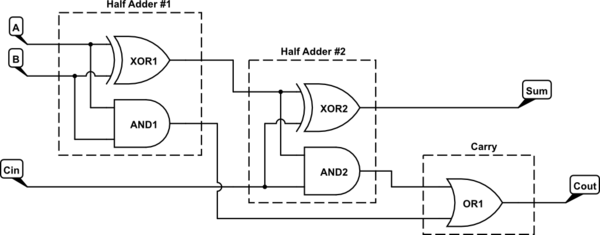
\includegraphics[width=0.8\textwidth, center]{./figures/HA_and_FA.png}
              \begin{itemize}
                \item es spielt beim FA bei der Verwendung keine Rolle, welches der 3 Inputs eigentlich für das Carry vorgesehen ist
              \end{itemize}
            \end{minipage}
          }
        }
      }
      child {
        node {Carry-Ripple-Addierer
          \resizebox{\textwidth}{!}{
            \begin{minipage}[t]{12cm}
              \begin{itemize}
                \item \href[page=341]{/home/areo/Documents/Studium/Summaries/Technische_Informatik/Technische_Informatik_all_in_one_with_go_back.pdf}{Definition}
                \item \href[page=346]{/home/areo/Documents/Studium/Summaries/Technische_Informatik/Technische_Informatik_all_in_one_with_go_back.pdf}{Kosten und Tiefe}
              \end{itemize}
              \begin{minipage}{0.3\textwidth}
                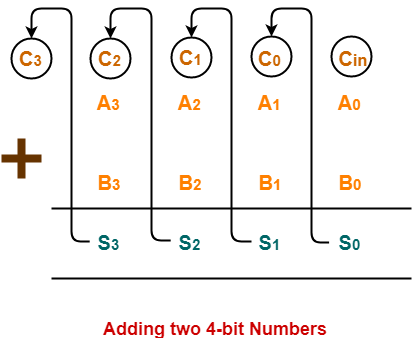
\includegraphics[width=\textwidth, center]{./figures/addition.png}
              \end{minipage}
              \begin{minipage}{0.7\textwidth}
                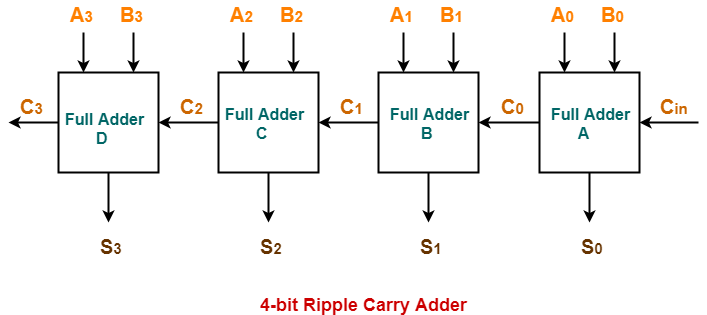
\includegraphics[width=\textwidth, center]{./figures/4_adder_substractor.png}
              \end{minipage}
              \begin{itemize}
                \item FA FA FA HA, wobei man allerdings meistens FA FA FA FA herstellt und das carry vom letzten FA unberührt lässt aber theoretisch Addierer zu größeren Addierern zusammenfügen kann
              \end{itemize}
            \end{minipage}
          }
        }
      }
          }
        }
    }
  }
    child {
      node {Sequentielle Logik}
    }
    child {
      node {Timing}
    };
  \end{scope}
  % ┌───────────────────┐
  % │ Verbindungslinien │
  % └───────────────────┘
  \begin{pgfonlayer}{background}
  % \draw [concept connection]
  %     (datahazardsforbranches) edge (forwarding);
  \end{pgfonlayer}
  % ┌──────────────┐
  % │ Annotationen │
  % └──────────────┘
  % https://tex.stackexchange.com/questions/302976/node-positioning-middle-point-mind-map-connection-bar
  \node [annotation, below] at (ti.south) {This mindmap is provided without guarantee of correctness and completeness!};
  \node [annotation, below] at (ti.north) {\href{/tmp/current.pdf}{go back}};
  \end{tikzpicture}
\end{document}
